\begin{figure}
  \centering
  \subcaptionbox{分图 A\label{fig:subfig-a}}
    {
\includegraphics[width=0.35\linewidth]{example-image-a.pdf}}
  \subcaptionbox{分图 B\label{fig:subfig-b}}
    {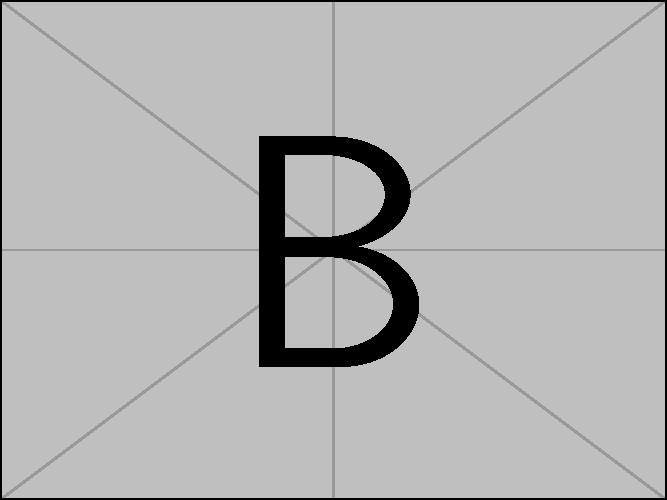
\includegraphics[width=0.35\linewidth]{example-image-b.pdf}}
  \caption{多个分图的示例}
  \label{fig:multi-image}
\end{figure}

\begin{table}
  \centering
  \begin{threeparttable}[c]
    \caption{带附注的表格示例}
    \label{tab:three-part-table}
    \begin{tabular}{ll}
      \toprule
      文件名                 & 描述                         \\
      \midrule
      thuthesis.dtx\tnote{a} & 模板的源文件,包括文档和注释 \\
      thuthesis.cls\tnote{b} & 模板文件                     \\
      thuthesis-*.bst        & BibTeX 参考文献表样式文件    \\
      \bottomrule
    \end{tabular}
    \begin{tablenotes}
      \item [a] 可以通过 xelatex 编译生成模板的使用说明文档;
        使用 xetex 编译 \file{thuthesis.ins} 时则会从 \file{.dtx} 中去除掉文档和注释,得到精简的 \file{.cls} 文件。
      \item [b] 更新模板时,一定要记得编译生成 \file{.cls} 文件,否则编译论文时载入的依然是旧版的模板。
    \end{tablenotes}
  \end{threeparttable}
\end{table}

\begin{longtable}{cccc}
    \caption{跨页长表格的表题} \\
    \toprule
    表头 1 & 表头 2 & 表头 3 & 表头 4 \\
    \midrule
  \endfirsthead
    \caption[]{跨页长表格的表题(续)} \\
    \toprule
    表头 1 & 表头 2 & 表头 3 & 表头 4 \\
    \midrule
  \endhead
    \bottomrule
  \endfoot
  Row 1  & & & \\
  Row 2  & & & \\
  Row 3  & & & \\
  Row 4  & & & \\
  Row 5  & & & \\
  Row 6  & & & \\
  Row 7  & & & \\
  Row 8  & & & \\
  Row 9  & & & \\
  Row 10 & & & \\
\end{longtable}

\section{算法}

算法环境可以使用 \pkg{algorithms} 或者 \pkg{algorithm2e} 宏包。

\renewcommand{\algorithmicrequire}{\textbf{输入:}\unskip}
\renewcommand{\algorithmicensure}{\textbf{输出:}\unskip}

\begin{algorithm}
  \caption{Calculate $y = x^n$}
  \label{alg1}
  \small
  \begin{algorithmic}
    \REQUIRE $n \geq 0$
    \ENSURE $y = x^n$

    \STATE $y \leftarrow 1$
    \STATE $X \leftarrow x$
    \STATE $N \leftarrow n$

    \WHILE{$N \neq 0$}
      \IF{$N$ is even}
        \STATE $X \leftarrow X \times X$
        \STATE $N \leftarrow N / 2$
      \ELSE[$N$ is odd]
        \STATE $y \leftarrow y \times X$
        \STATE $N \leftarrow N - 1$
      \ENDIF
    \ENDWHILE
  \end{algorithmic}
\end{algorithm}
